\chapter{提案モデルによる日本近辺の風速予測\label{chap:experiments}}
本論文では,提案モデルの性能検証のために日本近辺の風速予測を実施した.また,性能の比較のためにCNNによるエンコーダ・デコーダとLSTMを用いたエンコーダ・デコーダモデルを実装し,それぞれのモデルの性能を比較した.

\section{実験の概要 \label{section:exp-overview}}
本実験では,提案モデルと\ref{subsection:exp-encoder-decoder-model}項で説明するエンコーダ・デコーダモデルの2つのモデルに3時刻分の時系列データを入力し,それぞれの3時間後の風速を予測するように訓練した.その学習と評価には,\ref{section:exp-data-and-condition}節で述べるように気象庁が提供している日本近辺の風速と気圧データを用いた.

モデルが出力した最終時刻の予測値と実測値を用いて,以下の評価指標を算出した.ここで,指標に用いられる「風速」はベクトル量ではなく,スカラー量であることに注意されたい.
% 学習するLBM
% 学習しないLBM
% エンコーダ・デコーダ
% で,
% 全体のRMSE, ME
% 座標ごとのRMSE, ME 風速, 風向 %todo 東西方向, 南北方向
% 時間ごとのRMSE, ME 上のそれぞれ % todo
% 特徴的な日の座標のRMSE, ME 上のそれぞれ % todo
% 
% それぞれのRMSE比についても書く(4.4のほうかな?)
\begin{enumerate}
  \item 全体の風速の$\mathrm{RMSE[m/s]}$(Root Mean Squared Error, 二乗平均平方根誤差)と提案モデルのRMSE改善率[\%]
  \item 全体の風速の$\mathrm{ME[m/s]}$(Mean Error, 平均誤差)
  \item 全体の風向の$\mathrm{RMSE[^\circ]}$と提案モデルのRMSE改善率[\%]
  \item 座標ごとの風速の$\mathrm{RMSE[m/s]}$と提案モデルのRMSE改善率[\%]
  \item 座標ごとの風速の$\mathrm{ME[m/s]}$
  \item 座標ごとの風向の$\mathrm{RMSE[^\circ]}$と提案モデルのRMSE改善率[\%]
  % \item 時間ごとの風速のRMSEと提案モデルの改善率 %todo
  % \item 時間ごとの風速のME
  % \item 時間ごとの風向のRMSEと提案モデルの改善率
  % \item 時間ごとの風向のME
\end{enumerate}
これらの評価指標は一般的に気象予報モデルの統計的検証に用いられるものを参考にした\cite{Kishochou2018}.以下にRMSE改善率以外のそれぞれの評価指標の定義を示す.

\begin{equation}
  (\mathrm{全体の風速のRMSE [m/s]}) = \sqrt{\frac{1}{NM} \sum_{\bm{x}, i} (|\bm{w}(\bm{x}, t_i)| - |\hat{\bm{w}}(\bm{x}, t_i)|)^2}
  \label{eq:exp-rmse}
\end{equation}
\begin{equation}
  (\mathrm{全体の風速のME [m/s]}) = \frac{1}{NM} \sum_{\bm{x}, i} (|\bm{w}(\bm{x}, t_i)| - |\hat{\bm{w}}(\bm{x}, t_i)|)
  \label{eq:exp-me}
\end{equation}
\begin{equation}
  (\mathrm{全体の風向のRMSE [^\circ]}) = \sqrt{\frac{1}{NM} \sum_{\bm{x}, i} \mathrm{arg}(\bm{w}(\bm{x}, t_i), \hat{\bm{w}}(\bm{x}, t_i))^2}
  \label{eq:exp-rmse-direction}
\end{equation}
\begin{equation}
  (\mathrm{座標ごとの風速のRMSE [m/s]}) = \sqrt{\frac{1}{N} \sum_{\bm{i}} (|\bm{w}(\bm{x}, t_i)| - |\hat{\bm{w}}(\bm{x}, t_i)|)^2}
  \label{eq:exp-rmse-per-point}
\end{equation}
\begin{equation}
  (\mathrm{座標ごとの風速のME [m/s]}) = \frac{1}{N} \sum_{\bm{i}} (|\bm{w}(\bm{x}, t_i)| - |\hat{\bm{w}}(\bm{x}, t_i)|)
  \label{eq:exp-me-per-point}
\end{equation}
\begin{equation}
  (\mathrm{座標ごとの風向のRMSE [^\circ]}) = \sqrt{\frac{1}{N} \sum_{\bm{i}} \mathrm{arg}(\bm{w}(\bm{x}, t_i), \hat{\bm{w}}(\bm{x}, t_i))^2}
  \label{eq:exp-rmse-direction-per-point}
\end{equation}
ただし,$M$は格子点$\bm{x}$の総数,$N$はデータセットの総数とし,そのうちの$i$番目のデータセットについて$\bm{w}(\bm{x}, t_i)$をモデルによる予測風速ベクトル,$\hat{\bm{w}}(\bm{x}, t_i)$を実測の風速ベクトルとした.ここで,$\bm{w}(\bm{x}, t_i)$と$\hat{\bm{w}}(\bm{x}, t_i)$は共に速度の次元を持つ.また,$\mathrm{arg}$は二つのベクトルが成す角度を返す関数である.

また,RMSE改善率は以下の式で定義される.
\begin{equation}
  (\mathrm{RMSE改善率 [\%]}) = \frac{\mathrm{RMSE_{u-net}} - \mathrm{RMSE_{prop}}}{\mathrm{RMSE_{u-net}}} \times 100
  \label{eq:exp-rmse-improvement-rate}
\end{equation}
ただし,$\mathrm{RMSE_{u-net}}$はエンコーダ・デコーダモデルのRMSE,$\mathrm{RMSE_{prop}}$は提案モデルのRMSEを表す.

% 風速の時間変化を考慮せず,直前の風速をそのまま予測値とするPersistenceモデル

\section{利用したデータ及び学習条件 \label{section:exp-data-and-condition}}
\subsection{利用したデータ \label{subsection:exp-data}}
気象庁が提供している日本近辺の風速と気圧データを京都大学の生存圏データベース\cite{Seizonken2004}から入手した.このデータセットは図\ref{fig:exp-data-overview}に示す通り,日本近辺の北緯$22.4\tcdegree$から$47.6\tcdegree$まで,東経$120\tcdegree$から$150\tcdegree$までの領域をそれぞれ$0.05\tcdegree \times 0.0625\tcdegree$の細かさで等緯度等経度に区切り,各格子点上における風速と気圧を記録したものである\cite{JMBSC2022}.すなわち,ある一時刻のデータは緯度経度について$505 \times 480$の行列となっており,ある一点には風速の南北方向成分$[\mathrm{m/s}]$, 風速の東西方向成分$[\mathrm{m/s}]$, 気圧$[\mathrm{hPa}]$の3つの値が記録されている.
\begin{figure}[bp]
  \centering
  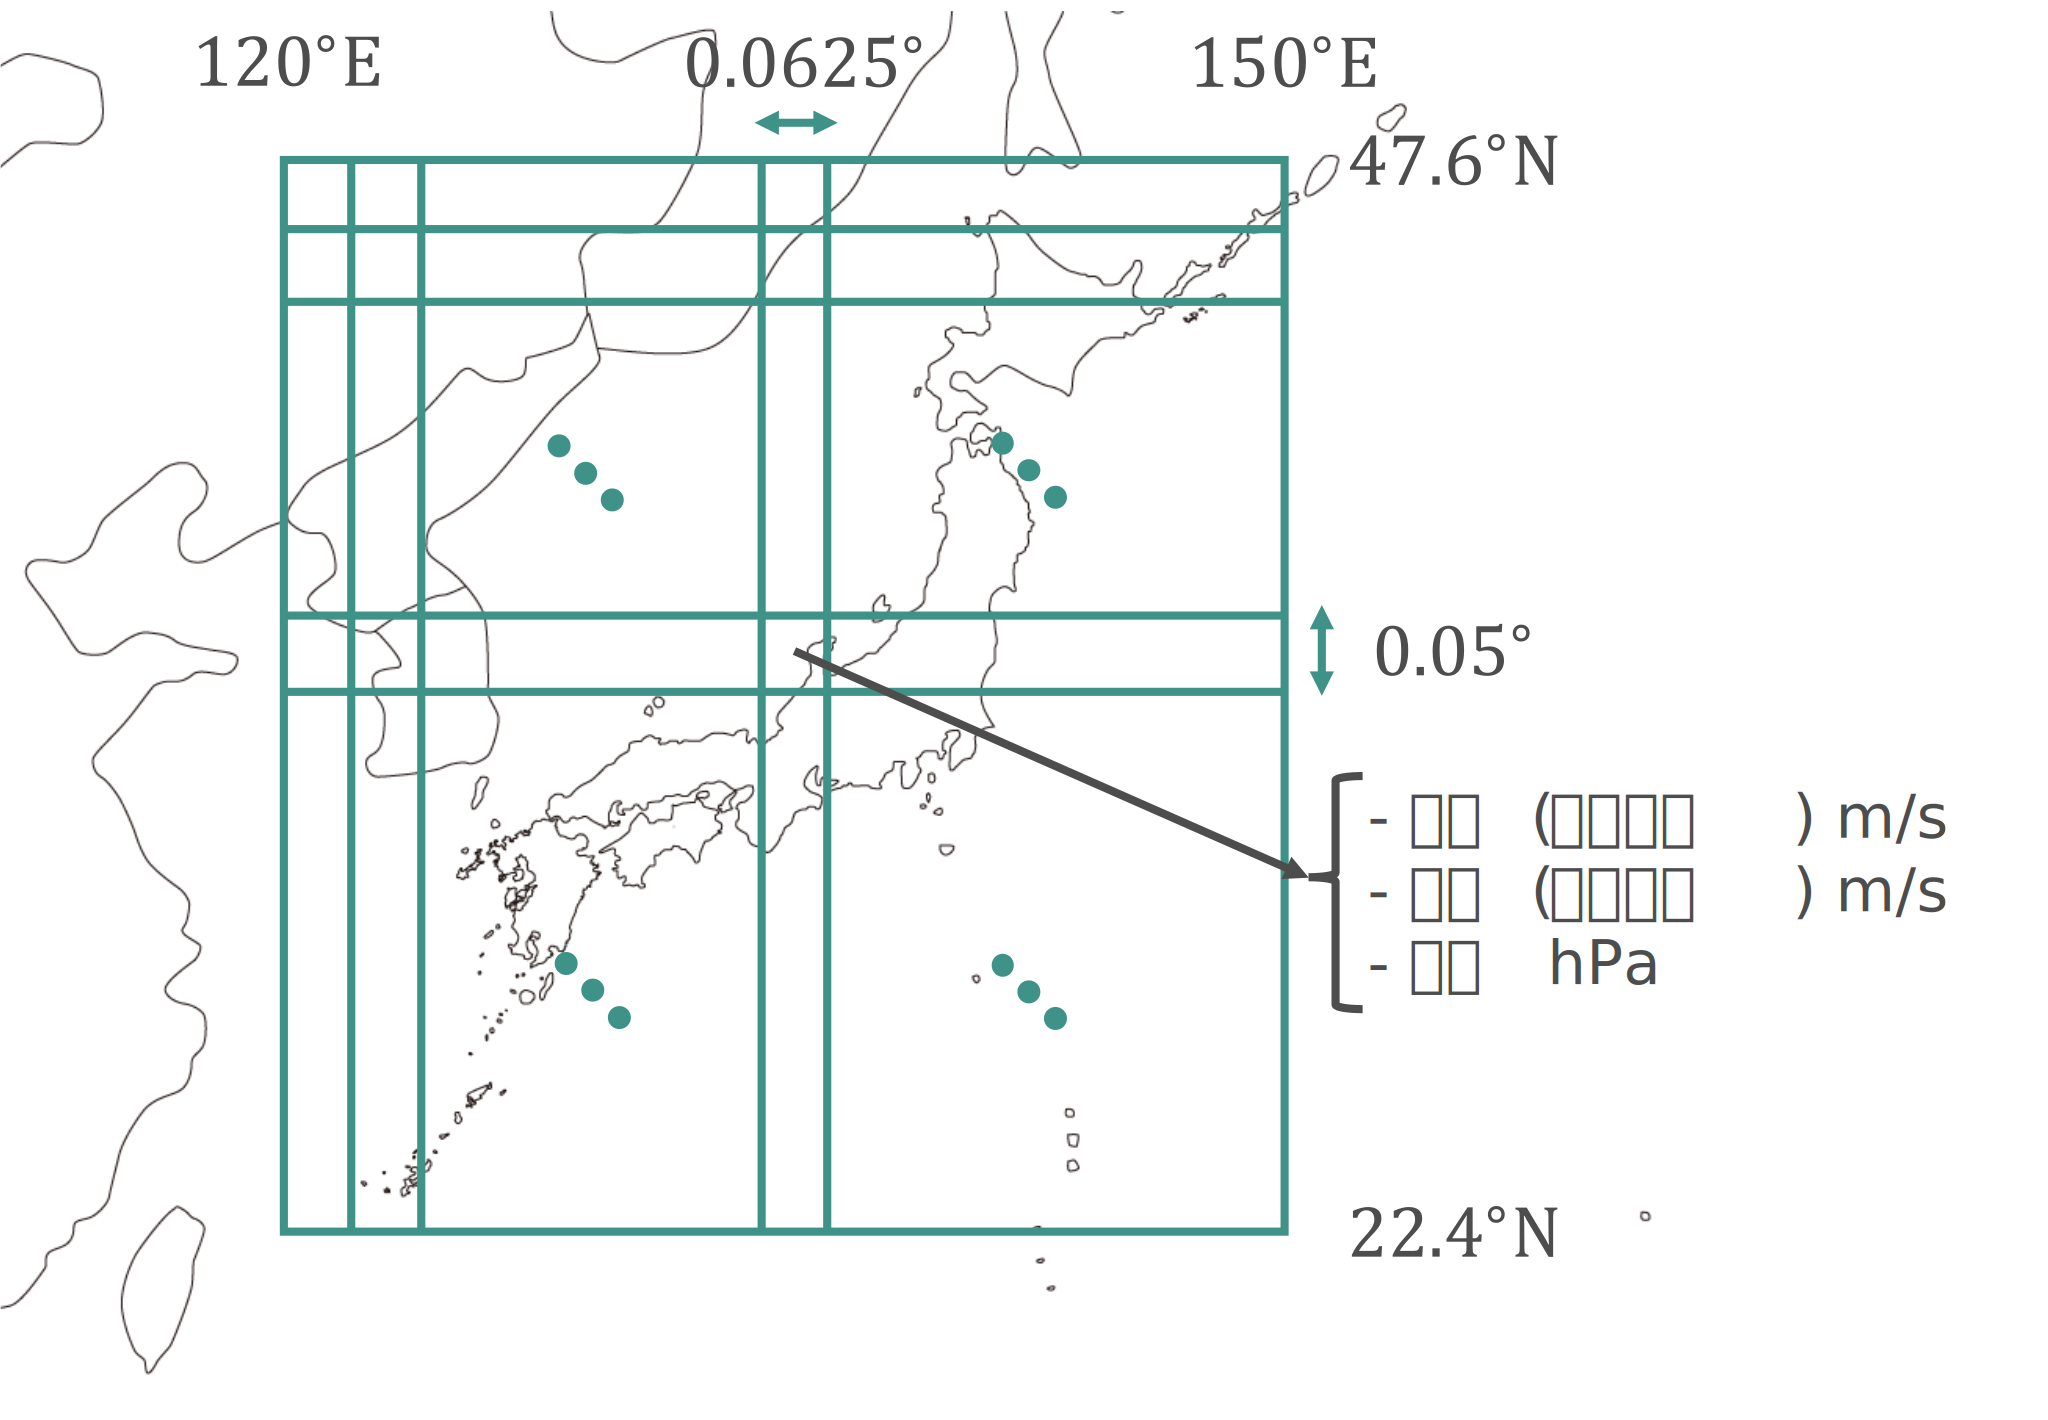
\includegraphics[width=0.6\linewidth]{./experiments/figs/data_overview.svg.eps}
  \caption{気象庁が提供している日本近辺の風速と気圧データの領域}
  \label{fig:exp-data-overview}
\end{figure}

提供されているデータは3時間間隔であり,(前日の)21:00, 0:00, 3:00, 6:00の4時刻分をひとまとめにして時系列データとした.これを2011年1月1日から2020年12月31日までの3650日分用意し(統計を取る際の簡便化のために閏日は除いてある),\ref{subsection:exp-data-preprocessing}項で述べる処理をする前の全体のデータセットとした.

%処理前の全体のデータセットの詳細な統計量を表\ref{todo:table:exp-pre-data-statistics}に示す.

\subsection{データの前処理 \label{subsection:exp-data-preprocessing}}
\ref{subsection:exp-data}項で述べたデータセットをそのまま入出力に用いるのではなく,前処理を実施した.その処理の詳細を以下に示す.

図\ref{fig:exp-averaging}に示すように,$505 \times 480$の行列を更に$10 \times 10$の格子によって区切り,この格子内で風速と気圧を平均化することで$50 \times 48$のサイズまで落とした.なお,端数分は切り捨てている.これは,提案モデルの格子の大きさを適切に設定することで,3時間で変化する風速の空間的な変化を捉えることができると考えたためである.このデータセットを改めて全体のデータセットとした.%このデータセットの詳細な統計量を表\ref{todo:table:exp-data-statistics}に示す.

\begin{figure}[bp]
  \centering
  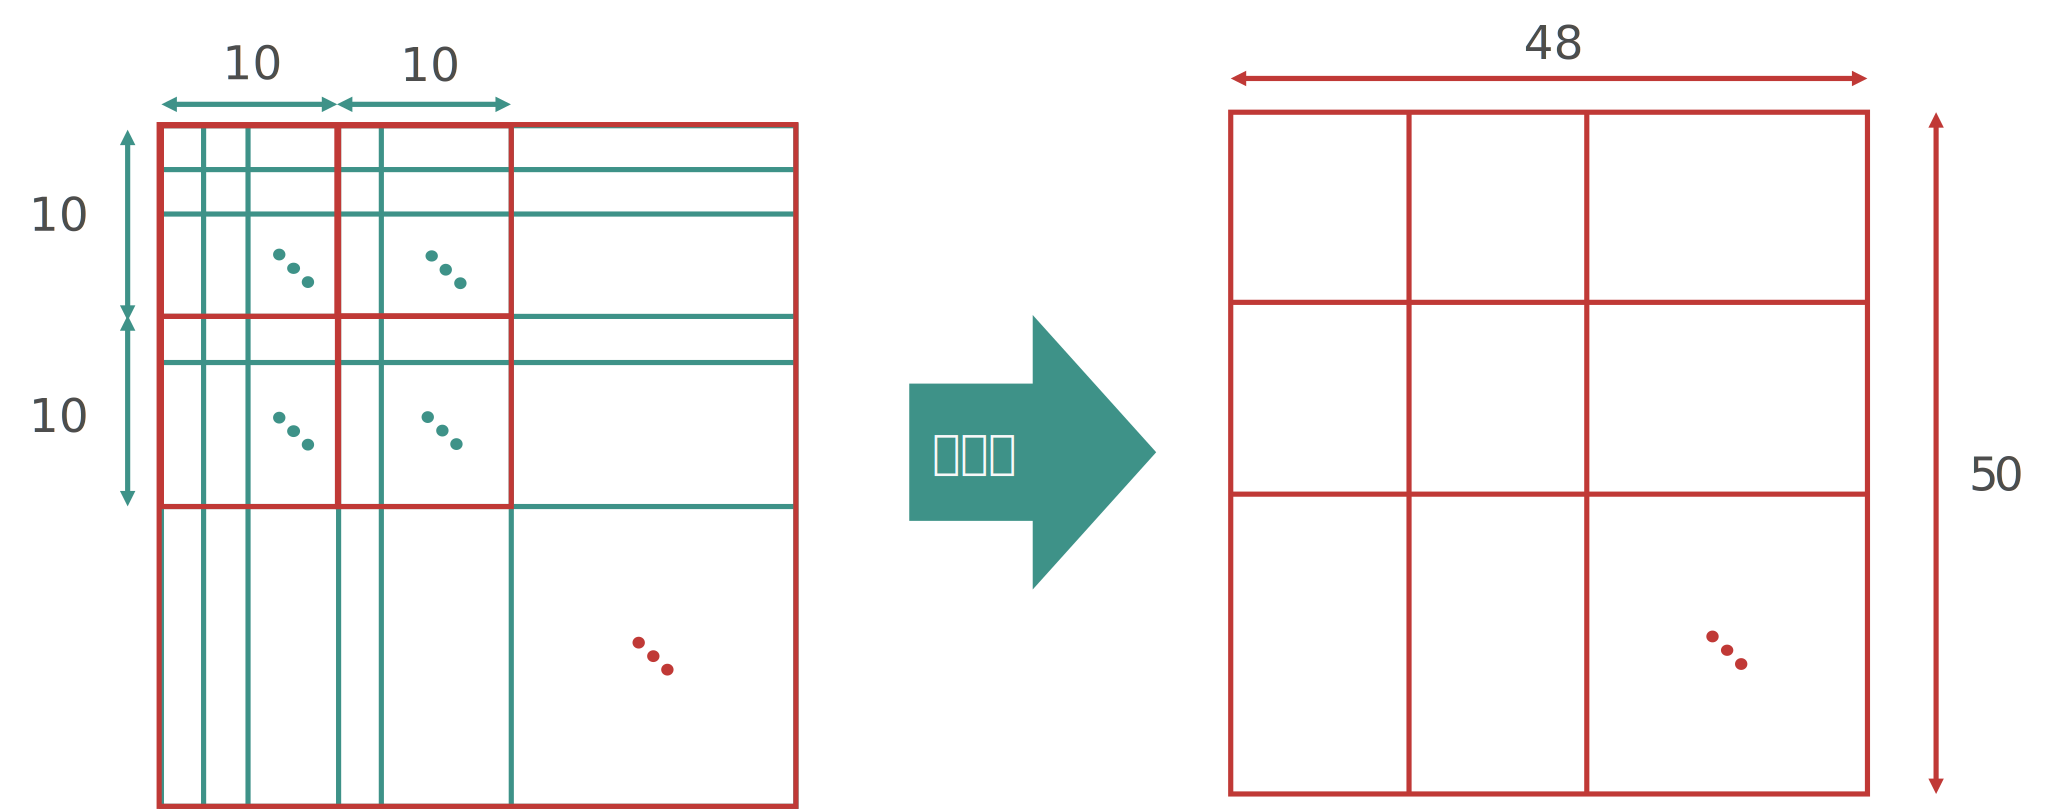
\includegraphics[width=0.8\linewidth]{./experiments/figs/average_pool.svg.eps}
  \caption{風速と気圧の平均化}
  \label{fig:exp-averaging}
\end{figure}

%todo 標準化についても時間があればここで触れる

\subsection{学習条件 \label{subsection:exp-condition}}

続いて,モデルの詳細な学習条件について述べる.提案モデルのアーキテクチャについての概要を\ref{subsection:time-series-model}項で述べたがここではより具体的に数値を提示し,モデルの仕様を詳細化する.図\ref{fig:exp-model-architecture}に示したように,このモデルでは並進と衝突をそれぞれ5回行った(緑の実線矢印が並進を表し,緑の破線矢印が衝突を表している).すなわち式(\ref{eq:time-series-t})において$\Delta T = 5$である.\ref{subsection:time-series-less-model}項で述べた通り衝突の回数分だけ外枠が削られるため,図中の赤破線によって強調されているように出力層の大きさは入力層に比べて東西南北の端$5$マス分減少している.
(前日の)21:00, 0:00, 3:00の3時刻分のデータを入力として0:00, 3:00, 6:00の風速を予測させた.すなわち,式(\ref{eq:time-series-input})において$n=4$,式(\ref{eq:time-series-t})において無次元時刻$\Delta T$は$3[\mathrm{h}]$相当である.

\begin{figure}[bp]
  \centering
  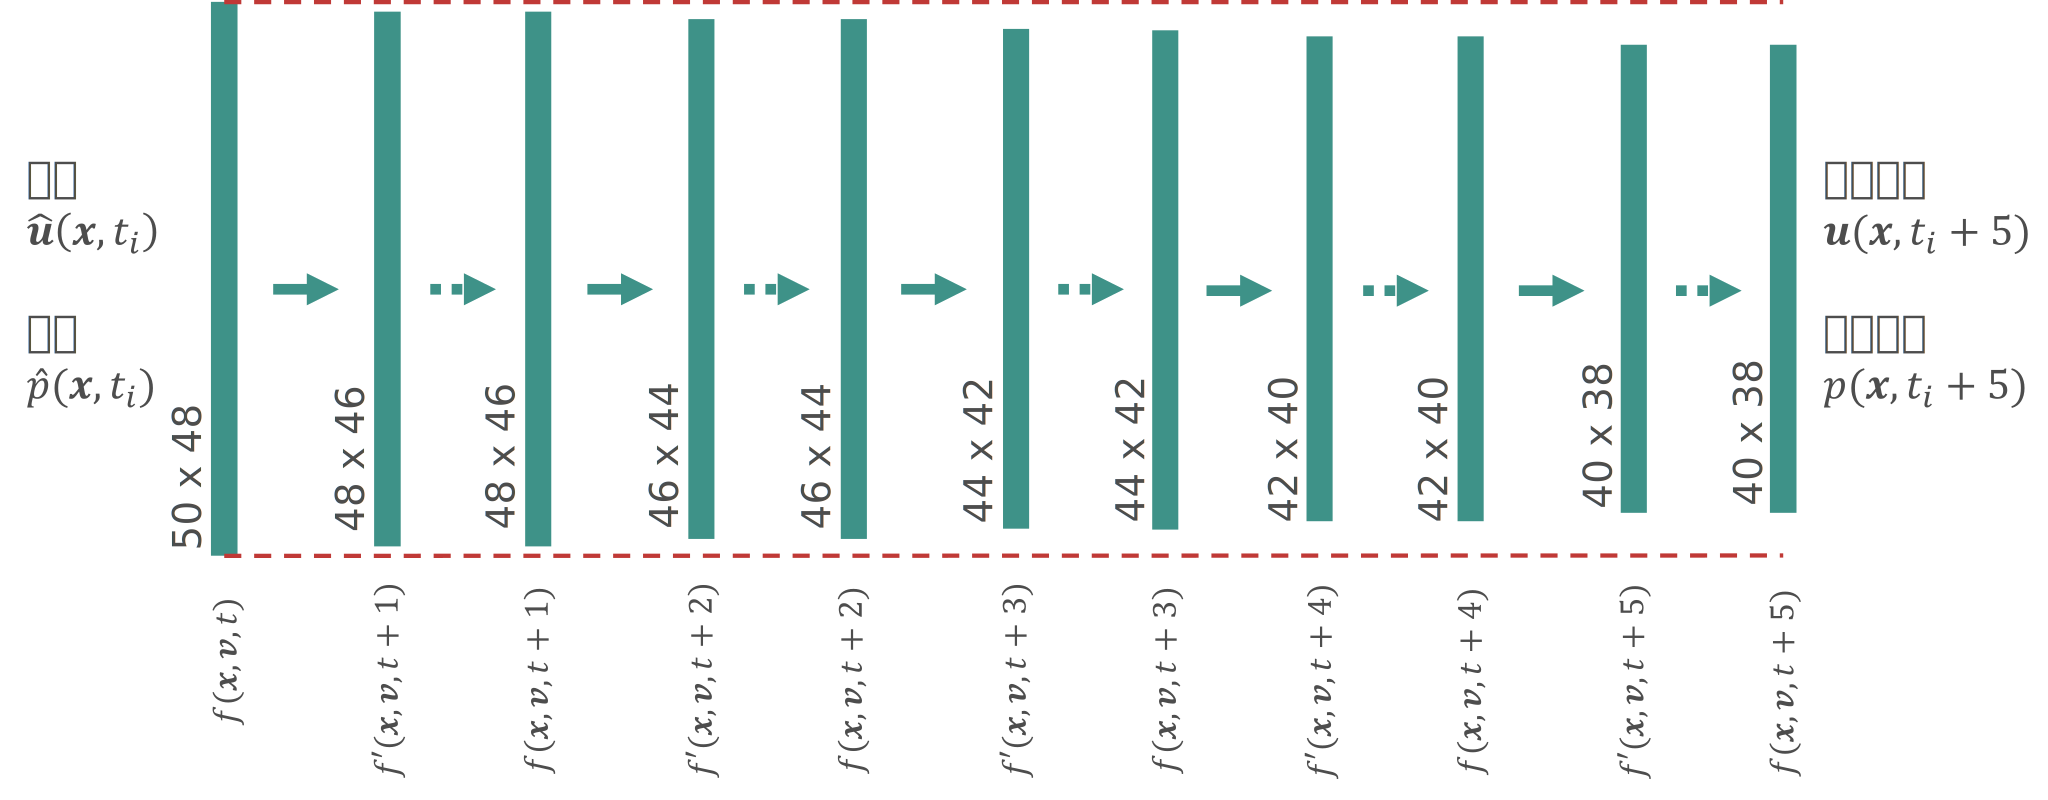
\includegraphics[width=0.85\linewidth]{./experiments/figs/model_architecture.svg.eps}
  \caption{モデルのアーキテクチャ}
  \label{fig:exp-model-architecture}
\end{figure}

% 損失関数について,式(\ref{eq:time-series-loss})に示したがここでは風速の精度を重視するため,式(\ref{eq:time-series-loss})の第1項の重みを$1$,第2項の重みを$0.1$とした.
%todo: なんで気圧の予測はしないのか聞かれたらこの辺も追記する

提案モデルの学習にはAdam\cite{Kingma2014AdamAM}を用いた.学習率は$10^{-3}$とし,ミニバッチサイズは$16$とした.全体のデータセットを2920日分と730日分に分けそれぞれを学習用データと検証用データとした.学習は$500$エポック行い,かかった時間は約8時間であった.実行環境にはGoogle Colaboratory\cite{GoogleColaboratory}を用い,GPUはTesla T4を用いた.また提案モデルの構築にはPyTorch\cite{NEURIPS2019-9015}を用い,自動微分による学習を行った.
% 損失の重み付けについて書く(速度に重みを強くつけた)

\section{実験結果 \label{section:exp-results}}
\ref{section:exp-overview}節で述べた評価指標を用いて,提案モデルの性能を評価した.その結果を順に述べる.
提案モデルの全体の風速の$\mathrm{RMSE[m/s]}$, $\mathrm{ME[m/s]}$はそれぞれ$1.0432\mathrm{[m/s]}$, $-0.1909\mathrm{[m/s]}$であった.提案モデルの全体の風向の$\mathrm{RMSE[^\circ]}$は$21.444\mathrm{[^\circ]}$であった.また,提案モデルの座標ごとの風速の$\mathrm{RMSE[m/s]}$, $\mathrm{ME[m/s]}$と風向の$\mathrm{RMSE[^\circ]}$はそれぞれ図\ref{fig:exp-speed-rmse-per-point}(a), \ref{fig:exp-speed-ma-per-point}(a), \ref{fig:exp-direction-rmse-per-point}(a)に示す通りであった.

\section{物理的な構造を含まない深層学習モデルによる実験結果 \label{section:exp-results-without-physicial-structure}}

\subsection{物理的な構造を含まない深層学習モデル \label{subsection:exp-encoder-decoder-model}}
提案モデルと比較するために用いた物理的な構造をもたないエンコーダ・デコーダモデルを図\ref{fig:exp-encoder-decoder-model}に示す.このモデルは\ref{subsec:chen2021}項で述べたChenらのモデルとU-Net\cite{journals/corr/RonnebergerFB15}を参考にしたものである.図中の各層の左に大きさを,上部にチャンネル数を記載してある.入出力部分では,風速の東西方向成分と南北方向成分,そして気圧を正規化して3チャンネルにまとめた.エンコーダ・デコーダの各層には畳み込み層とバッチ正規化\cite{10.5555/3045118.3045167},活性化関数である$\tanh$を用いた.また,エンコーダの各層の出力をコピーしてデコーダの対応する層の入力に結合するスキップコネクションを用いた.エンコーダから出力される信号を平滑化してからLSTMユニットに入力し,その出力をデコーダに入力した.デコードの際にはサイズを復元するために逆畳み込み層を用いた.出力の際に,提案モデルと性能比較をできるように周囲5マス分を切り捨てた.

\begin{figure}[bp]
  \centering
  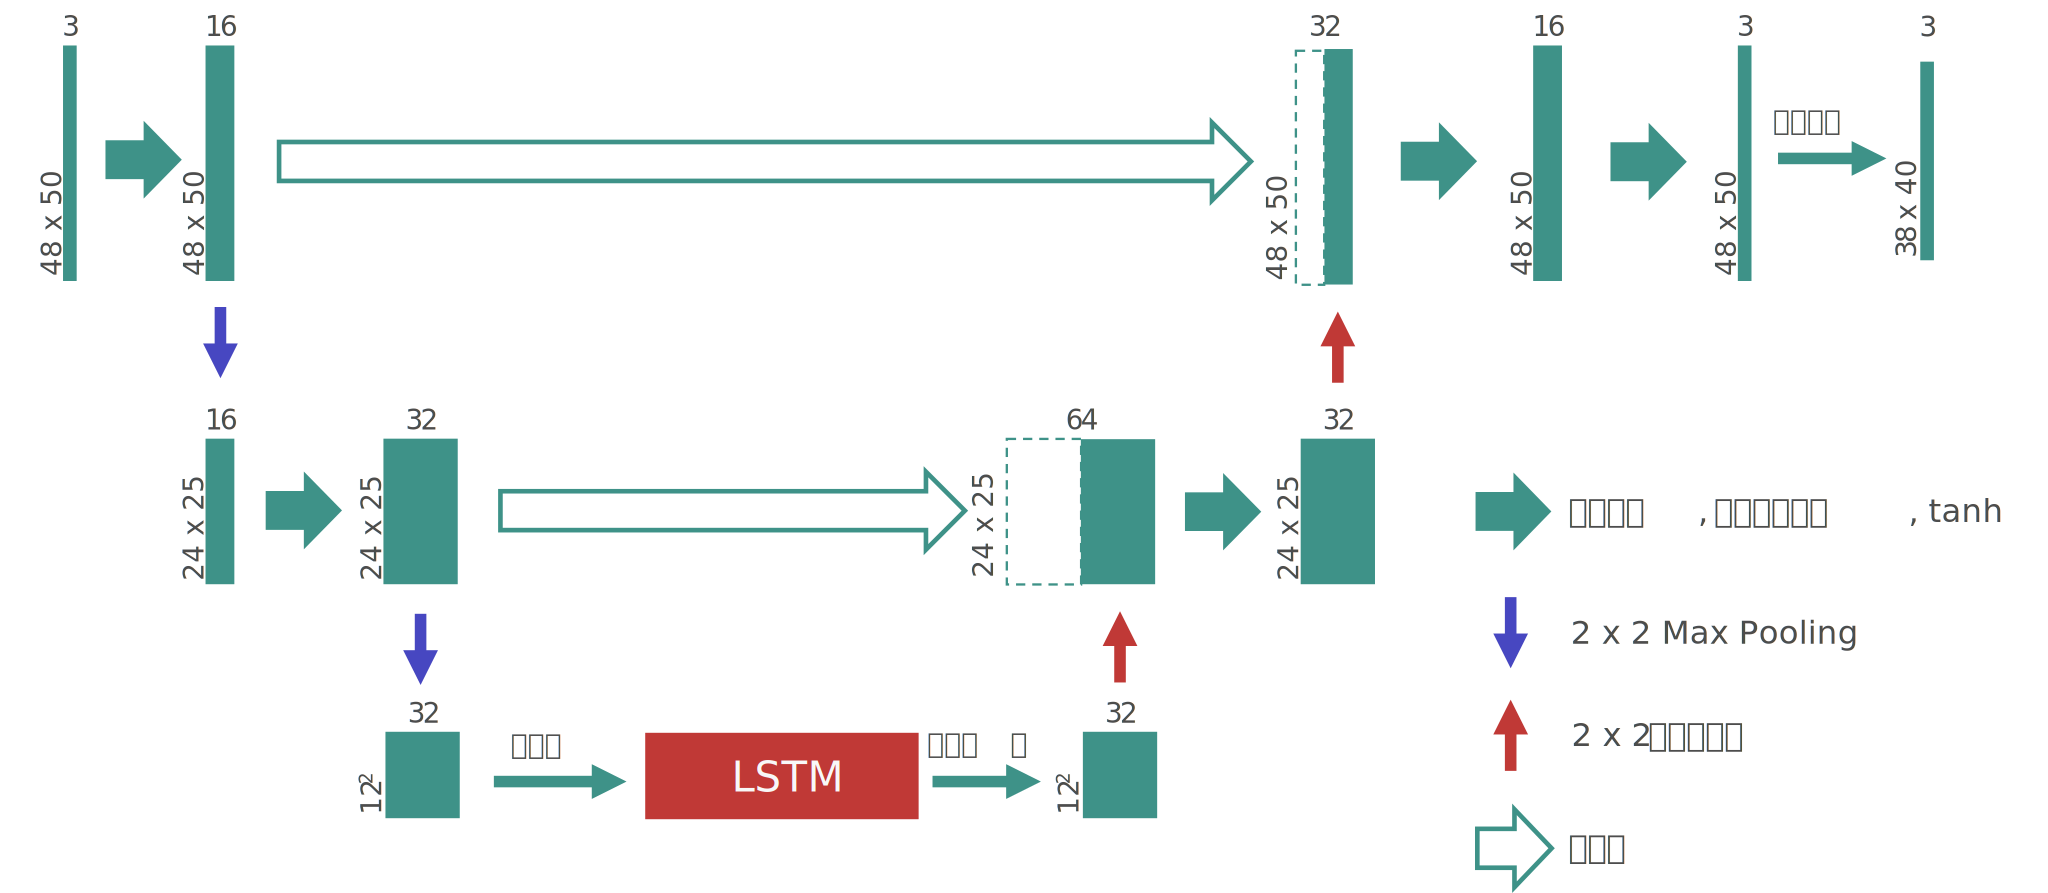
\includegraphics[width=0.9\linewidth]{./experiments/figs/u_net_like_model_architecture.svg.eps}
  \caption{物理的な構造を含まない深層学習モデルのアーキテクチャ}
  \label{fig:exp-encoder-decoder-model}
\end{figure}

その他の利用したデータ及び学習条件は\ref{section:exp-data-and-condition}節と同様である.

\subsection{実験結果 \label{subsection:exp-results-without-physicial-structure}}
\ref{section:exp-overview}節で述べた評価指標を用いて,エンコーダ・デコーダモデルの性能を評価し,提案モデルと比較した.
エンコーダ・デコーダモデルについて,全体の風速の$\mathrm{RMSE[m/s]}$と$\mathrm{ME[m/s]}$,そして風向の$\mathrm{RMSE[^\circ]}$をそれぞれ提案モデルの結果と比較しながら,それぞれ表\ref{table:exp-total-rmse}に示す.また,座標ごとの風速の$\mathrm{RMSE[m/s]}$と$\mathrm{ME[m/s]}$,そして風向の$\mathrm{RMSE[^\circ]}$をそれぞれ提案モデルの結果と比較しながら,それぞれ図\ref{fig:exp-speed-rmse-per-point}, \ref{fig:exp-speed-ma-per-point}, \ref{fig:exp-direction-rmse-per-point}に示す.

\begin{table}[bp]
  \caption{全体の風速の$\mathrm{RMSE[m/s]}$}
  \label{table:exp-total-rmse}
  \centering
  \begin{tabular}{ccc}
    \hline
    提案モデル & エンコーダ・デコーダモデル & RMSE改善率 \\
    \hline
    1.0432 & 1.0930 & 4.57 \\
    \hline
  \end{tabular}
\end{table}

\begin{table}[bp]
  \caption{全体の風速の$\mathrm{ME[m/s]}$}
  \label{table:exp-total-me}
  \centering
  \begin{tabular}{cc}
    \hline
    提案モデル & エンコーダ・デコーダモデル \\
    \hline
    -0.1909 & 0.2001 \\
    \hline
  \end{tabular}
\end{table}

\begin{table}[bp]
  \caption{全体の風向の$\mathrm{RMSE[^\circ]}$}
  \label{table:exp-total-direction-rmse}
  \centering
  \begin{tabular}{ccc}
    \hline
    提案モデル & エンコーダ・デコーダモデル & RMSE改善率 \\
    \hline
    21.444 & 22.521 & 4.78 \\
    \hline
  \end{tabular}
\end{table}

\begin{figure}[bp]
  \centering
  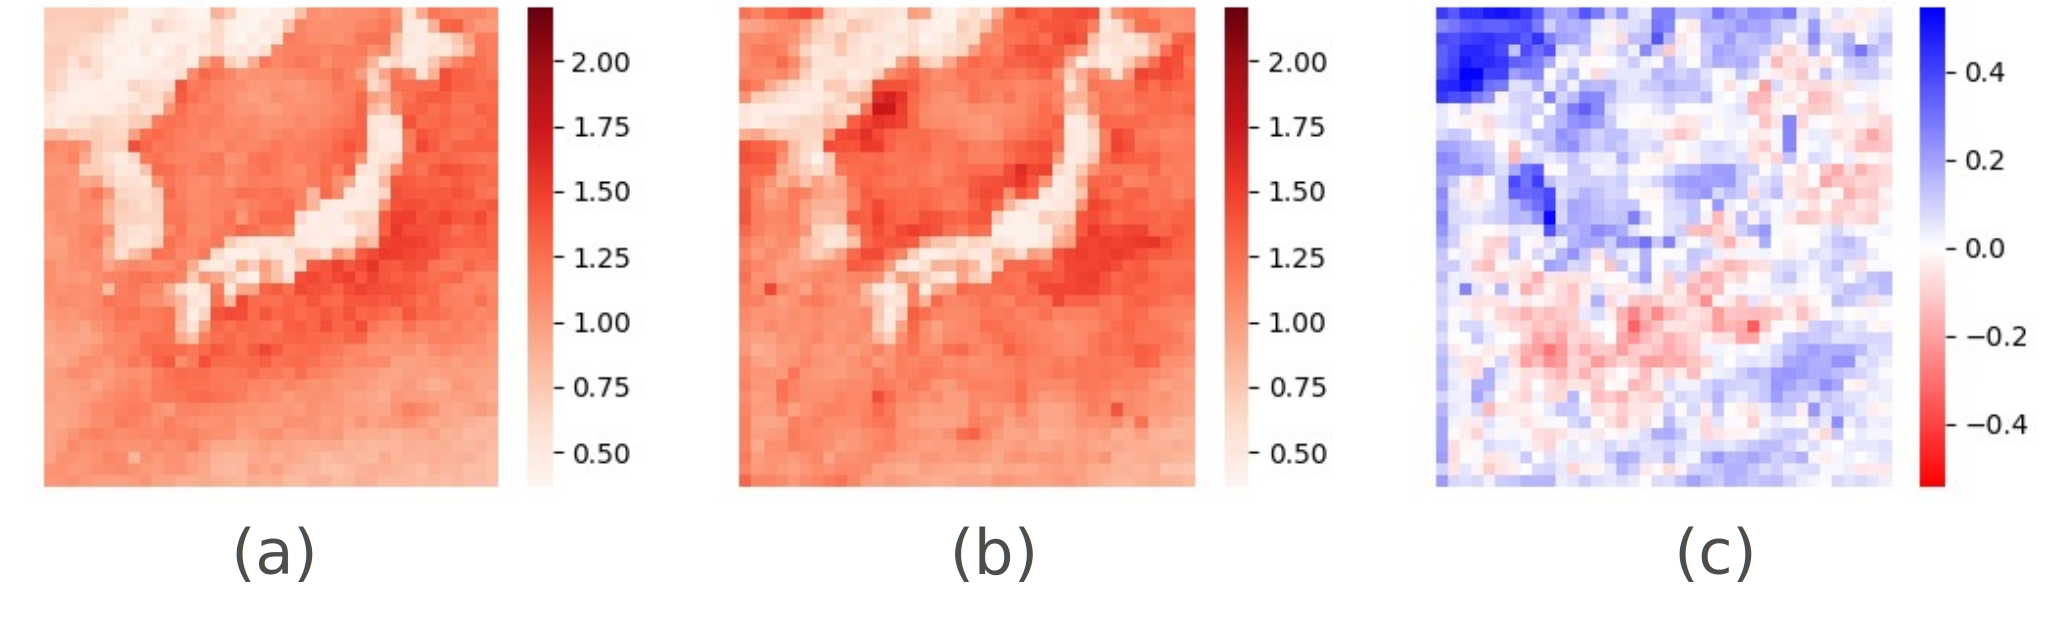
\includegraphics[width=0.9\linewidth]{./experiments/figs/result_speed_rmse_per_point.svg.eps}
  \caption{座標ごとの風速のRMSE[m/s] (a)提案モデルの$\mathrm{RMSE[m/s]}$ (b)エンコーダ・デコーダモデルの$\mathrm{RMSE[m/s]}$ (c)提案モデルによる$\mathrm{RMSE改善率[\%]}$}
  \label{fig:exp-speed-rmse-per-point}
\end{figure}

\begin{figure}[bp]
  \centering
  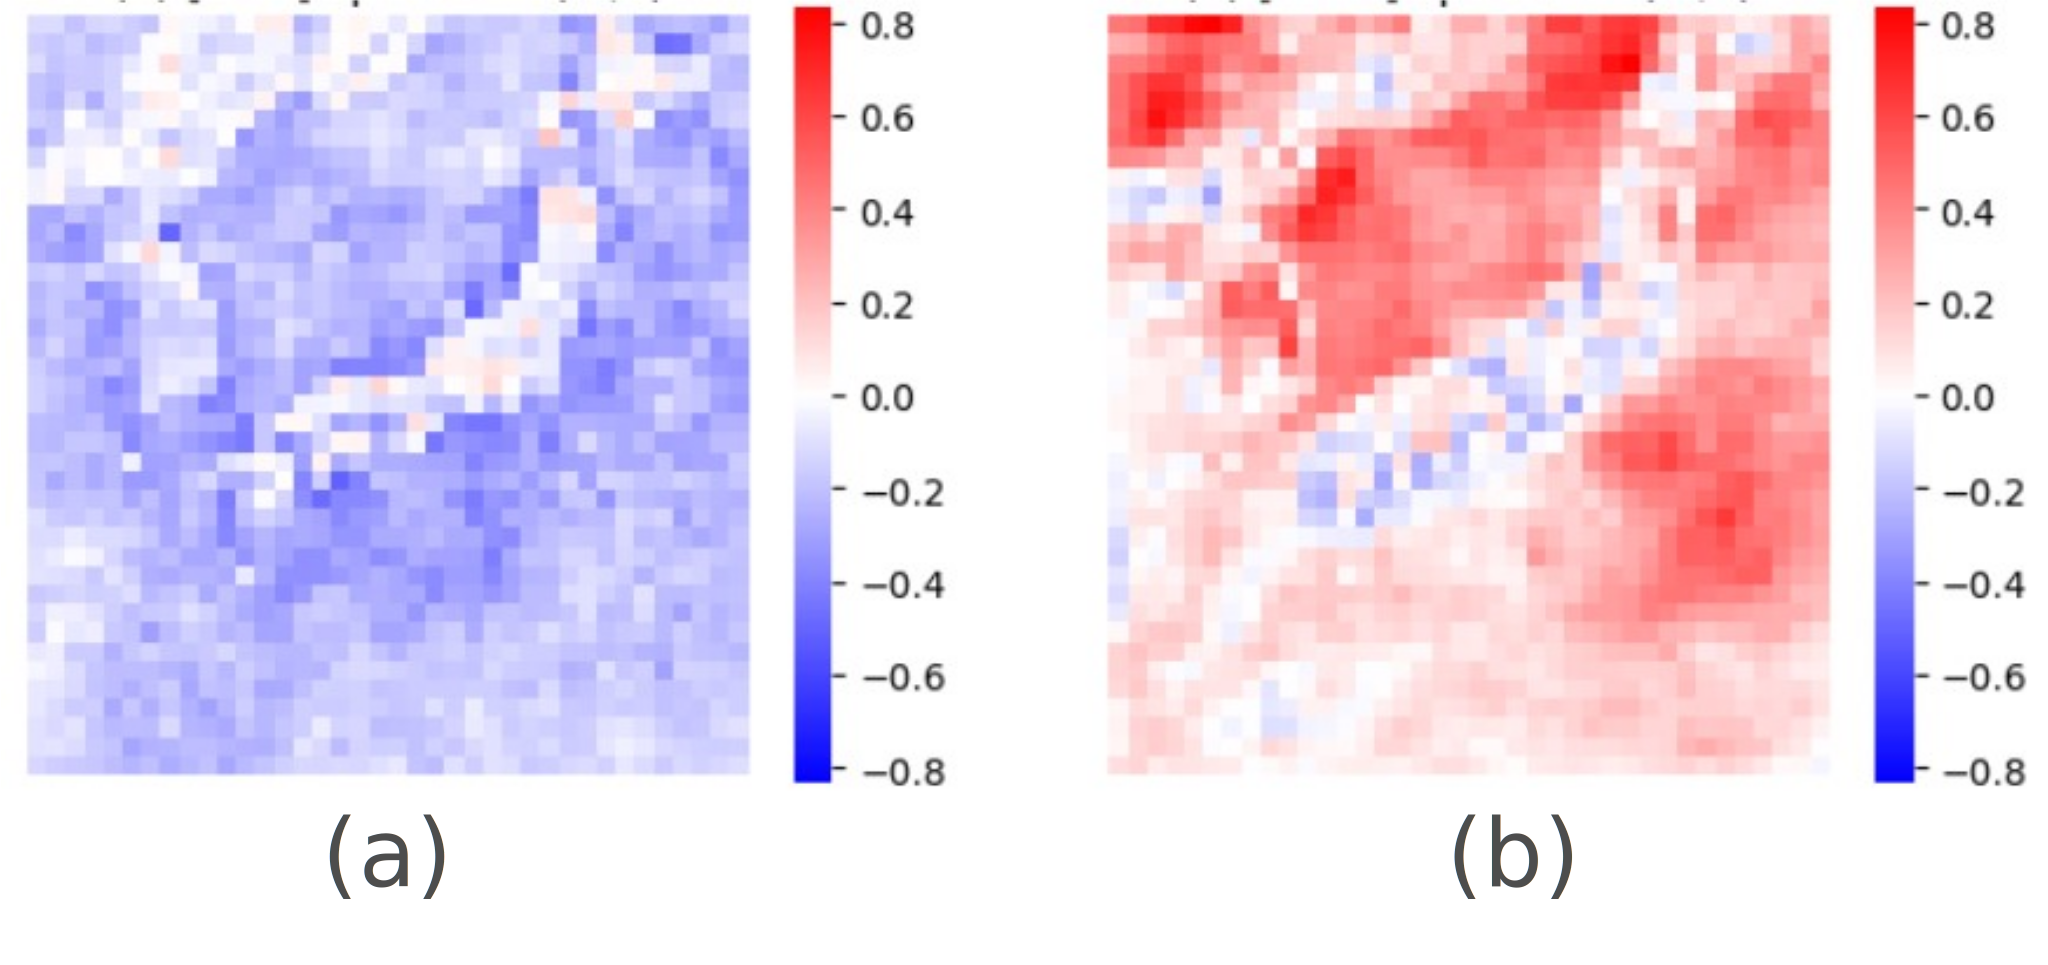
\includegraphics[width=0.6\linewidth]{./experiments/figs/result_speed_me_per_point.svg.eps}
  \caption{座標ごとの風速の$\mathrm{ME[m/s]}$ (a)提案モデルの$\mathrm{ME[m/s]}$ (b)エンコーダ・デコーダモデルの$\mathrm{ME[m/s]}$}
  \label{fig:exp-speed-ma-per-point}
\end{figure}

\begin{figure}[bp]
  \centering
  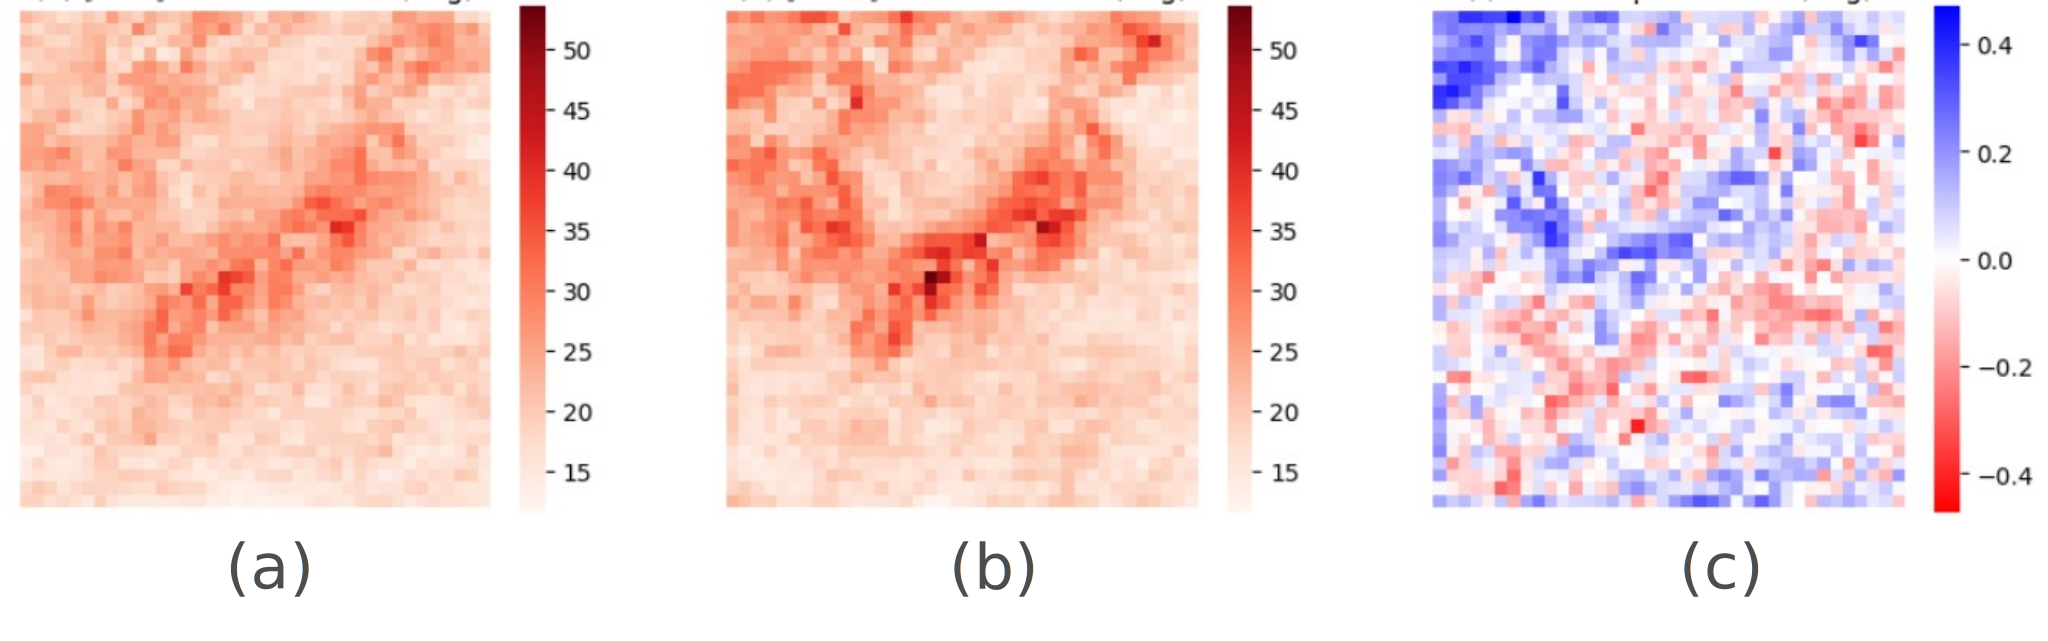
\includegraphics[width=0.9\linewidth]{./experiments/figs/result_direction_rmse_per_point.svg.eps}
  \caption{座標ごとの風向の$\mathrm{RMSE[^\circ]}$ (a)提案モデルの$\mathrm{RMSE[^\circ]}$ (b)エンコーダ・デコーダモデルの$\mathrm{RMSE[^\circ]}$ (c)提案モデルによるRMSE改善率$\mathrm{[\%]}$}
  \label{fig:exp-direction-rmse-per-point}
\end{figure}

\section{考察 \label{section:exp-discussion}}
表\ref{table:exp-total-direction-rmse}と表\ref{table:exp-total-rmse}より,$\mathrm{RMSE改善率[\%]}$が0より真に大きいことから,提案モデルの方がエンコーダ・デコーダモデルよりも風速と風向の予測精度が高いことがわかった.これにより,提案モデルの大局的な優位性を示すことができた.以下,提案モデルとエンコーダ・デコーダモデルの予測精度の共通点と相違点から,日本近辺の大気の性質及び二つのモデルの性質について考察する.

図\ref{fig:exp-speed-rmse-per-point}(a),(b)をみると,2つのモデルは共に陸上よりも海上の風速誤差の方が大きいことがわかった.これに対して,図\ref{fig:exp-direction-rmse-per-point}(a),(b)をみると,2つのモデルは共に海上よりも陸上の風向誤差の方が大きいことがわかった.これは,海上は遮蔽物が存在しないため風速が陸上よりも大きい傾向にありその分変化量も大きいこと,そして陸上の風向は複雑な地形によって海上よりも変化量が大きくなることが原因として考えられる.

表\ref{table:exp-total-me}及び図\ref{fig:exp-speed-ma-per-point}(a)から,提案モデルは風速を小さく見積もる傾向があることがわかった.これは,提案モデルが衝突のプロセスによって平衡に向かう性質があるためだと言える.これに対して,表\ref{table:exp-total-me}及び図\ref{fig:exp-speed-ma-per-point}(b)より,エンコーダ・デコーダモデルは風速を大きく見積もる傾向があることがわかった.これは活性化関数の$\tanh$が原点近傍で大きな傾きをもち,そこから離れると傾きが小さくなるため,バッチ正規化によって入力が原点近傍に集まることで風速を大きく見積もる傾向があると考えられる.

最後に,図\ref{fig:exp-speed-rmse-per-point}(c)と図\ref{fig:exp-direction-rmse-per-point}(c)をみると,提案モデルはエンコーダ・デコーダモデルに比べて陸上では精度が改善し陸と海の境界付近で精度が悪化することがわかった.これは,提案モデルが座標に依存性のある陸上の風速変化を捉えることができているのに対し,エンコーダ・デコーダモデルは境界の特徴を捉えることができていることを示唆する.

% 提案モデルの優位性を示すことができた ok
% 風速の誤差は海上のほうがおおきい ok
% 風向の誤差は陸上のほうがおおきい ok
% 提案モデルは風速を小さく見積もりがち ok
% エンコーダ・デコーダモデルは風速を大きく見積もりがち ok
% 提案モデルは陸上ではよくて大陸と海の境界付近で誤差が大きい ok
% 平均化についてもふれて,どうやってアップスケーリングするか 
% 短所として外枠の風速が予測できないことにふれる